\documentclass[1p]{elsarticle_modified}
%\bibliographystyle{elsarticle-num}

%\usepackage[colorlinks]{hyperref}
%\usepackage{abbrmath_seonhwa} %\Abb, \Ascr, \Acal ,\Abf, \Afrak
\usepackage{amsfonts}
\usepackage{amssymb}
\usepackage{amsmath}
\usepackage{amsthm}
\usepackage{scalefnt}
\usepackage{amsbsy}
\usepackage{kotex}
\usepackage{caption}
\usepackage{subfig}
\usepackage{color}
\usepackage{graphicx}
\usepackage{xcolor} %% white, black, red, green, blue, cyan, magenta, yellow
\usepackage{float}
\usepackage{setspace}
\usepackage{hyperref}

\usepackage{tikz}
\usetikzlibrary{arrows}

\usepackage{multirow}
\usepackage{array} % fixed length table
\usepackage{hhline}

%%%%%%%%%%%%%%%%%%%%%
\makeatletter
\renewcommand*\env@matrix[1][\arraystretch]{%
	\edef\arraystretch{#1}%
	\hskip -\arraycolsep
	\let\@ifnextchar\new@ifnextchar
	\array{*\c@MaxMatrixCols c}}
\makeatother %https://tex.stackexchange.com/questions/14071/how-can-i-increase-the-line-spacing-in-a-matrix
%%%%%%%%%%%%%%%

\usepackage[normalem]{ulem}

\newcommand{\msout}[1]{\ifmmode\text{\sout{\ensuremath{#1}}}\else\sout{#1}\fi}
%SOURCE: \msout is \stkout macro in https://tex.stackexchange.com/questions/20609/strikeout-in-math-mode

\newcommand{\cancel}[1]{
	\ifmmode
	{\color{red}\msout{#1}}
	\else
	{\color{red}\sout{#1}}
	\fi
}

\newcommand{\add}[1]{
	{\color{blue}\uwave{#1}}
}

\newcommand{\replace}[2]{
	\ifmmode
	{\color{red}\msout{#1}}{\color{blue}\uwave{#2}}
	\else
	{\color{red}\sout{#1}}{\color{blue}\uwave{#2}}
	\fi
}

\newcommand{\Sol}{\mathcal{S}} %segment
\newcommand{\D}{D} %diagram
\newcommand{\A}{\mathcal{A}} %arc


%%%%%%%%%%%%%%%%%%%%%%%%%%%%%5 test

\def\sl{\operatorname{\textup{SL}}(2,\Cbb)}
\def\psl{\operatorname{\textup{PSL}}(2,\Cbb)}
\def\quan{\mkern 1mu \triangleright \mkern 1mu}

\theoremstyle{definition}
\newtheorem{thm}{Theorem}[section]
\newtheorem{prop}[thm]{Proposition}
\newtheorem{lem}[thm]{Lemma}
\newtheorem{ques}[thm]{Question}
\newtheorem{cor}[thm]{Corollary}
\newtheorem{defn}[thm]{Definition}
\newtheorem{exam}[thm]{Example}
\newtheorem{rmk}[thm]{Remark}
\newtheorem{alg}[thm]{Algorithm}

\newcommand{\I}{\sqrt{-1}}
\begin{document}

%\begin{frontmatter}
%
%\title{Boundary parabolic representations of knots up to 8 crossings}
%
%%% Group authors per affiliation:
%\author{Yunhi Cho} 
%\address{Department of Mathematics, University of Seoul, Seoul, Korea}
%\ead{yhcho@uos.ac.kr}
%
%
%\author{Seonhwa Kim} %\fnref{s_kim}}
%\address{Center for Geometry and Physics, Institute for Basic Science, Pohang, 37673, Korea}
%\ead{ryeona17@ibs.re.kr}
%
%\author{Hyuk Kim}
%\address{Department of Mathematical Sciences, Seoul National University, Seoul 08826, Korea}
%\ead{hyukkim@snu.ac.kr}
%
%\author{Seokbeom Yoon}
%\address{Department of Mathematical Sciences, Seoul National University, Seoul, 08826,  Korea}
%\ead{sbyoon15@snu.ac.kr}
%
%\begin{abstract}
%We find all boundary parabolic representation of knots up to 8 crossings.
%
%\end{abstract}
%\begin{keyword}
%    \MSC[2010] 57M25 
%\end{keyword}
%
%\end{frontmatter}

%\linenumbers
%\tableofcontents
%
\newcommand\colored[1]{\textcolor{white}{\rule[-0.35ex]{0.8em}{1.4ex}}\kern-0.8em\color{red} #1}%
%\newcommand\colored[1]{\textcolor{white}{ #1}\kern-2.17ex	\textcolor{white}{ #1}\kern-1.81ex	\textcolor{white}{ #1}\kern-2.15ex\color{red}#1	}

{\Large $\underline{12a_{0230}~(K12a_{0230})}$}

\setlength{\tabcolsep}{10pt}
\renewcommand{\arraystretch}{1.6}
\vspace{1cm}\begin{tabular}{m{100pt}>{\centering\arraybackslash}m{274pt}}
\multirow{5}{120pt}{
	\centering
	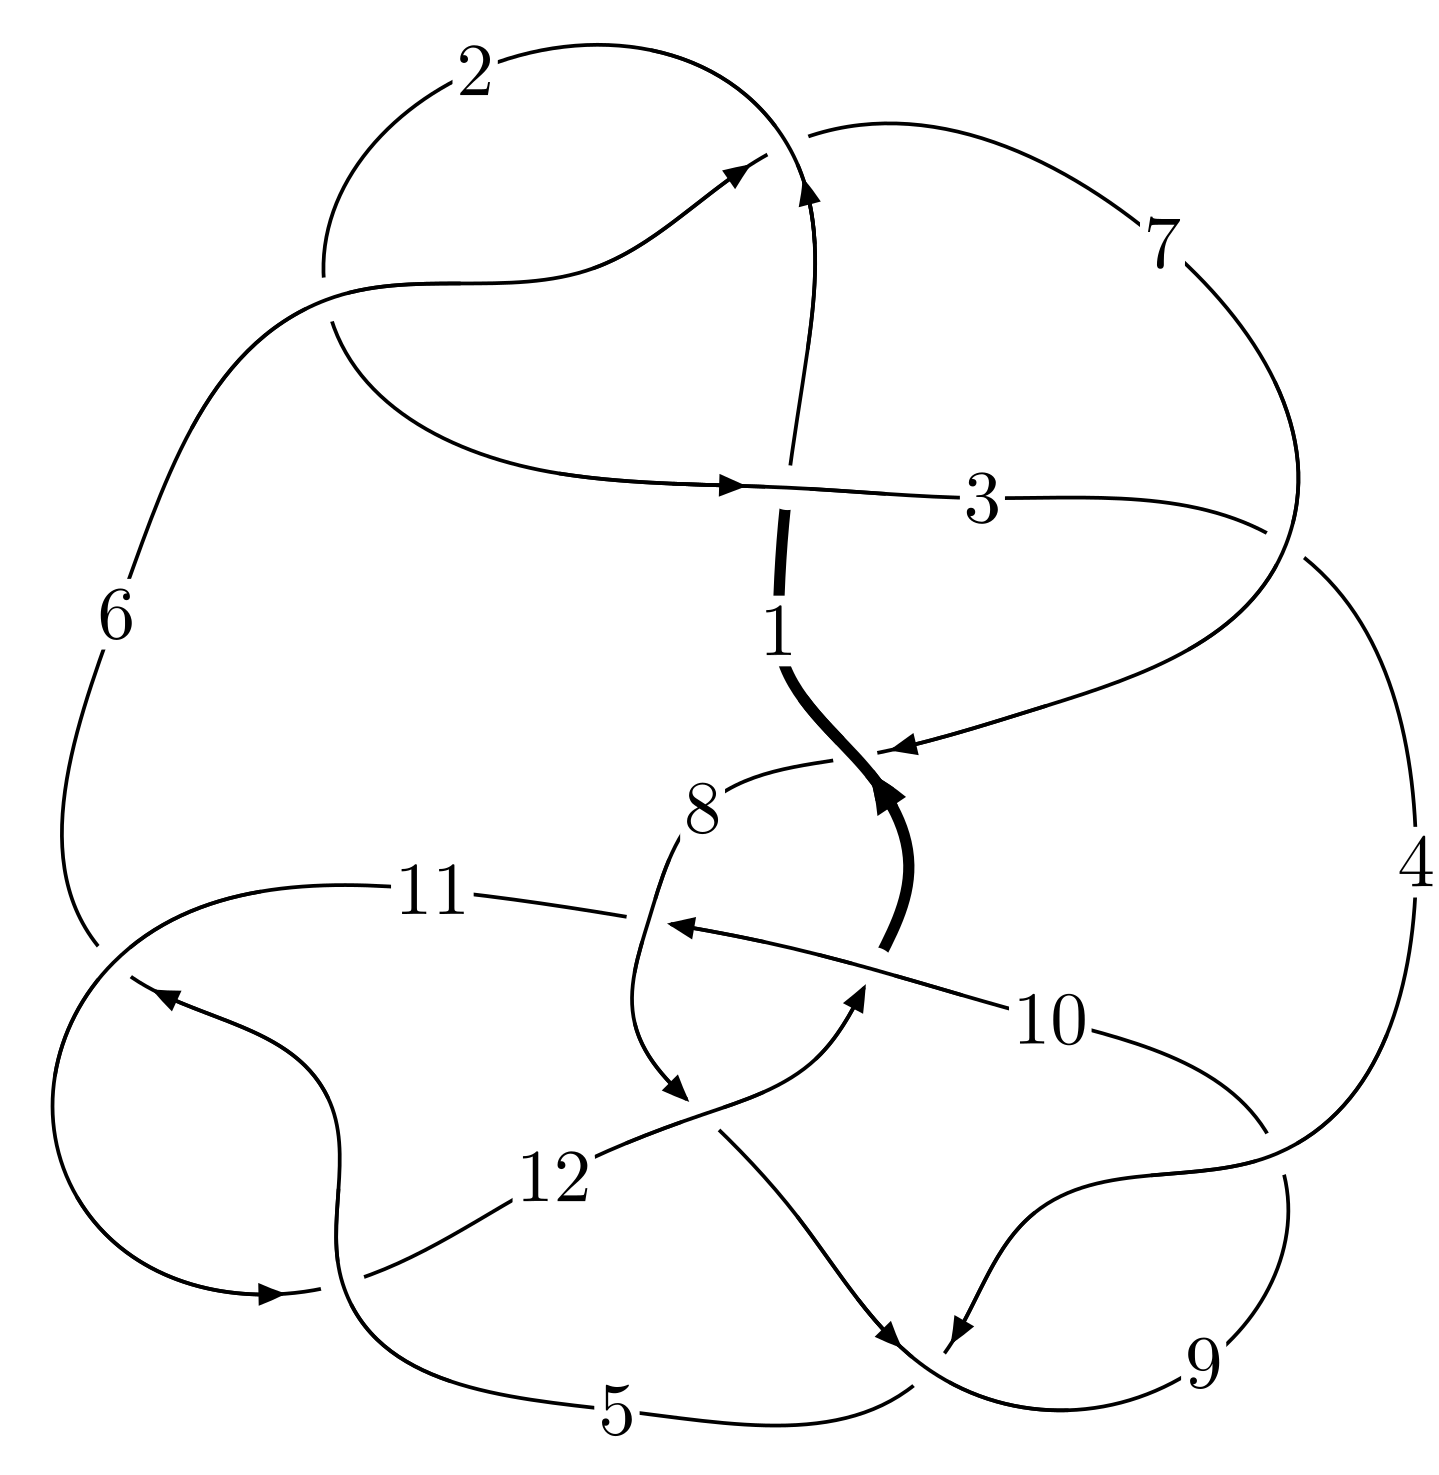
\includegraphics[width=112pt]{../../../GIT/diagram.site/Diagrams/png/1031_12a_0230.png}\\
\ \ \ A knot diagram\footnotemark}&
\allowdisplaybreaks
\textbf{Linearized knot diagam} \\
\cline{2-2}
 &
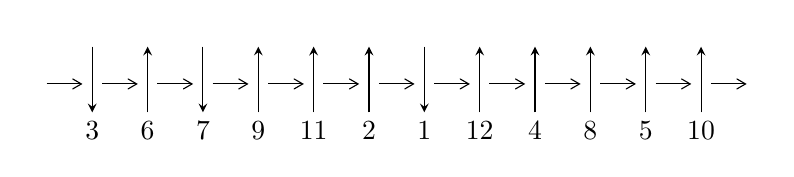
\begin{tikzpicture}[x=20pt, y=17pt]
	% nodes
	\node (C0) at (0, 0) {};
	\node (C1) at (1, 0) {};
	\node (C1U) at (1, +1) {};
	\node (C1D) at (1, -1) {3};

	\node (C2) at (2, 0) {};
	\node (C2U) at (2, +1) {};
	\node (C2D) at (2, -1) {6};

	\node (C3) at (3, 0) {};
	\node (C3U) at (3, +1) {};
	\node (C3D) at (3, -1) {7};

	\node (C4) at (4, 0) {};
	\node (C4U) at (4, +1) {};
	\node (C4D) at (4, -1) {9};

	\node (C5) at (5, 0) {};
	\node (C5U) at (5, +1) {};
	\node (C5D) at (5, -1) {11};

	\node (C6) at (6, 0) {};
	\node (C6U) at (6, +1) {};
	\node (C6D) at (6, -1) {2};

	\node (C7) at (7, 0) {};
	\node (C7U) at (7, +1) {};
	\node (C7D) at (7, -1) {1};

	\node (C8) at (8, 0) {};
	\node (C8U) at (8, +1) {};
	\node (C8D) at (8, -1) {12};

	\node (C9) at (9, 0) {};
	\node (C9U) at (9, +1) {};
	\node (C9D) at (9, -1) {4};

	\node (C10) at (10, 0) {};
	\node (C10U) at (10, +1) {};
	\node (C10D) at (10, -1) {8};

	\node (C11) at (11, 0) {};
	\node (C11U) at (11, +1) {};
	\node (C11D) at (11, -1) {5};

	\node (C12) at (12, 0) {};
	\node (C12U) at (12, +1) {};
	\node (C12D) at (12, -1) {10};
	\node (C13) at (13, 0) {};

	% arrows
	\draw[->,>={angle 60}]
	(C0) edge (C1) (C1) edge (C2) (C2) edge (C3) (C3) edge (C4) (C4) edge (C5) (C5) edge (C6) (C6) edge (C7) (C7) edge (C8) (C8) edge (C9) (C9) edge (C10) (C10) edge (C11) (C11) edge (C12) (C12) edge (C13) ;	\draw[->,>=stealth]
	(C1U) edge (C1D) (C2D) edge (C2U) (C3U) edge (C3D) (C4D) edge (C4U) (C5D) edge (C5U) (C6D) edge (C6U) (C7U) edge (C7D) (C8D) edge (C8U) (C9D) edge (C9U) (C10D) edge (C10U) (C11D) edge (C11U) (C12D) edge (C12U) ;
	\end{tikzpicture} \\
\hhline{~~} \\& 
\textbf{Solving Sequence} \\ \cline{2-2} 
 &
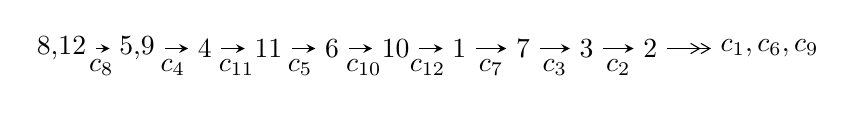
\begin{tikzpicture}[x=23pt, y=7pt]
	% node
	\node (A0) at (-1/8, 0) {8,12};
	\node (A1) at (17/16, 0) {5,9};
	\node (A2) at (17/8, 0) {4};
	\node (A3) at (25/8, 0) {11};
	\node (A4) at (33/8, 0) {6};
	\node (A5) at (41/8, 0) {10};
	\node (A6) at (49/8, 0) {1};
	\node (A7) at (57/8, 0) {7};
	\node (A8) at (65/8, 0) {3};
	\node (A9) at (73/8, 0) {2};
	\node (C1) at (1/2, -1) {$c_{8}$};
	\node (C2) at (13/8, -1) {$c_{4}$};
	\node (C3) at (21/8, -1) {$c_{11}$};
	\node (C4) at (29/8, -1) {$c_{5}$};
	\node (C5) at (37/8, -1) {$c_{10}$};
	\node (C6) at (45/8, -1) {$c_{12}$};
	\node (C7) at (53/8, -1) {$c_{7}$};
	\node (C8) at (61/8, -1) {$c_{3}$};
	\node (C9) at (69/8, -1) {$c_{2}$};
	\node (A10) at (11, 0) {$c_{1},c_{6},c_{9}$};

	% edge
	\draw[->,>=stealth]	
	(A0) edge (A1) (A1) edge (A2) (A2) edge (A3) (A3) edge (A4) (A4) edge (A5) (A5) edge (A6) (A6) edge (A7) (A7) edge (A8) (A8) edge (A9) ;
	\draw[->>,>={angle 60}]	
	(A9) edge (A10);
\end{tikzpicture} \\ 

\end{tabular} \\

\footnotetext{
The image of knot diagram is generated by the software ``\textbf{Draw programme}" developed by Andrew Bartholomew(\url{http://www.layer8.co.uk/maths/draw/index.htm\#Running-draw}), where we modified some parts for our purpose(\url{https://github.com/CATsTAILs/LinksPainter}).
}\phantom \\ \newline 
\centering \textbf{Ideals for irreducible components\footnotemark of $X_{\text{par}}$} 
 
\begin{align*}
I^u_{1}&=\langle 
-11158891 u^{48}-471894272 u^{47}+\cdots+4194304 b+6878327209984,\\
\phantom{I^u_{1}}&\phantom{= \langle  }-79952981 u^{48}-3436338262 u^{47}+\cdots+8388608 a-448987463155712,\\
\phantom{I^u_{1}}&\phantom{= \langle  }u^{49}+44 u^{48}+\cdots+201326592 u+8388608\rangle \\
I^u_{2}&=\langle 
-3.30457\times10^{120} a^{45} u+1.96555\times10^{120} a^{44} u+\cdots+2.43626\times10^{123} a-4.32752\times10^{122},\\
\phantom{I^u_{2}}&\phantom{= \langle  }- a^{45} u-12 a^{44} u+\cdots+633 a-110,\;u^2- u+1\rangle \\
I^u_{3}&=\langle 
-22 u^{23}-61 u^{22}+\cdots+b+41,\;-38 u^{23}-111 u^{22}+\cdots+a+59,\;u^{24}+3 u^{23}+\cdots-2 u+1\rangle \\
\\
\end{align*}
\raggedright * 3 irreducible components of $\dim_{\mathbb{C}}=0$, with total 165 representations.\\
\footnotetext{All coefficients of polynomials are rational numbers. But the coefficients are sometimes approximated in decimal forms when there is not enough margin.}
\newpage
\renewcommand{\arraystretch}{1}
\centering \section*{I. $I^u_{1}= \langle -1.12\times10^{7} u^{48}-4.72\times10^{8} u^{47}+\cdots+4.19\times10^{6} b+6.88\times10^{12},\;-8.00\times10^{7} u^{48}-3.44\times10^{9} u^{47}+\cdots+8.39\times10^{6} a-4.49\times10^{14},\;u^{49}+44 u^{48}+\cdots+201326592 u+8388608 \rangle$}
\flushleft \textbf{(i) Arc colorings}\\
\begin{tabular}{m{7pt} m{180pt} m{7pt} m{180pt} }
\flushright $a_{8}=$&$\begin{pmatrix}1\\0\end{pmatrix}$ \\
\flushright $a_{12}=$&$\begin{pmatrix}0\\u\end{pmatrix}$ \\
\flushright $a_{5}=$&$\begin{pmatrix}9.53114 u^{48}+409.643 u^{47}+\cdots+1.27596\times10^{9} u+5.35235\times10^{7}\\2.66049 u^{48}+112.508 u^{47}+\cdots-1.29286\times10^{7} u-1639921\end{pmatrix}$ \\
\flushright $a_{9}=$&$\begin{pmatrix}1\\- u^2\end{pmatrix}$ \\
\flushright $a_{4}=$&$\begin{pmatrix}-0.195494 u^{48}-11.2622 u^{47}+\cdots-5.89390\times10^{8} u-2.64295\times10^{7}\\5.17357 u^{48}+225.387 u^{47}+\cdots+1.32808\times10^{9} u+5.76352\times10^{7}\end{pmatrix}$ \\
\flushright $a_{11}=$&$\begin{pmatrix}-0.000244141 u^{48}-0.0107422 u^{47}+\cdots-48128 u-2047.50\\-0.000488281 u^{48}-0.0209961 u^{47}+\cdots-49151.5 u-2048\end{pmatrix}$ \\
\flushright $a_{6}=$&$\begin{pmatrix}14.0885 u^{48}+603.980 u^{47}+\cdots+1.57173\times10^{9} u+6.49774\times10^{7}\\-4.13982 u^{48}-186.093 u^{47}+\cdots-2.19280\times10^{9} u-9.69151\times10^{7}\end{pmatrix}$ \\
\flushright $a_{10}=$&$\begin{pmatrix}0.000244141 u^{48}+0.0102539 u^{47}+\cdots+1023.50 u+0.500000\\-0.000488281 u^{48}-0.0209961 u^{47}+\cdots-49151.5 u-2048\end{pmatrix}$ \\
\flushright $a_{1}=$&$\begin{pmatrix}-0.00219727 u^{48}-0.0959473 u^{47}+\cdots-386048. u-16384\\0.000732422 u^{48}+0.0346680 u^{47}+\cdots+425985 u+18432\end{pmatrix}$ \\
\flushright $a_{7}=$&$\begin{pmatrix}-0.0363770 u^{48}-1.54468 u^{47}+\cdots-1803264 u-70655\\0.0534668 u^{48}+2.30933 u^{47}+\cdots+7382016 u+311296\end{pmatrix}$ \\
\flushright $a_{3}=$&$\begin{pmatrix}34.9112 u^{48}+1497.44 u^{47}+\cdots+4.47944\times10^{9} u+1.88451\times10^{8}\\-14.8198 u^{48}-653.719 u^{47}+\cdots-5.04287\times10^{9} u-2.20698\times10^{8}\end{pmatrix}$ \\
\flushright $a_{2}=$&$\begin{pmatrix}13.8492 u^{48}+591.479 u^{47}+\cdots+1.33993\times10^{9} u+5.53213\times10^{7}\\-13.8870 u^{48}-602.707 u^{47}+\cdots-2.88876\times10^{9} u-1.24329\times10^{8}\end{pmatrix}$\\&\end{tabular}
\flushleft \textbf{(ii) Obstruction class $= -1$}\\~\\
\flushleft \textbf{(iii) Cusp Shapes $= \frac{1939025}{262144} u^{48}+\frac{175746237}{524288} u^{47}+\cdots+4242276468 u+187028462$}\\~\\
\newpage\renewcommand{\arraystretch}{1}
\flushleft \textbf{(iv) u-Polynomials at the component}\newline \\
\begin{tabular}{m{50pt}|m{274pt}}
Crossings & \hspace{64pt}u-Polynomials at each crossing \\
\hline $$\begin{aligned}c_{1}\end{aligned}$$&$\begin{aligned}
&u^{49}+24 u^{48}+\cdots+108 u-16
\end{aligned}$\\
\hline $$\begin{aligned}c_{2},c_{6}\end{aligned}$$&$\begin{aligned}
&u^{49}-6 u^{48}+\cdots+38 u-4
\end{aligned}$\\
\hline $$\begin{aligned}c_{3}\end{aligned}$$&$\begin{aligned}
&u^{49}+6 u^{48}+\cdots-2874 u-612
\end{aligned}$\\
\hline $$\begin{aligned}c_{4},c_{5},c_{9}\\c_{11}\end{aligned}$$&$\begin{aligned}
&u^{49}+17 u^{47}+\cdots+2 u-1
\end{aligned}$\\
\hline $$\begin{aligned}c_{7}\end{aligned}$$&$\begin{aligned}
&u^{49}-30 u^{48}+\cdots+42842 u-3676
\end{aligned}$\\
\hline $$\begin{aligned}c_{8}\end{aligned}$$&$\begin{aligned}
&u^{49}-44 u^{48}+\cdots+201326592 u-8388608
\end{aligned}$\\
\hline $$\begin{aligned}c_{10},c_{12}\end{aligned}$$&$\begin{aligned}
&u^{49}-2 u^{48}+\cdots-6 u-1
\end{aligned}$\\
\hline
\end{tabular}\\~\\
\newpage\renewcommand{\arraystretch}{1}
\flushleft \textbf{(v) Riley Polynomials at the component}\newline \\
\begin{tabular}{m{50pt}|m{274pt}}
Crossings & \hspace{64pt}Riley Polynomials at each crossing \\
\hline $$\begin{aligned}c_{1}\end{aligned}$$&$\begin{aligned}
&y^{49}+4 y^{48}+\cdots+26352 y-256
\end{aligned}$\\
\hline $$\begin{aligned}c_{2},c_{6}\end{aligned}$$&$\begin{aligned}
&y^{49}+24 y^{48}+\cdots+108 y-16
\end{aligned}$\\
\hline $$\begin{aligned}c_{3}\end{aligned}$$&$\begin{aligned}
&y^{49}-10 y^{48}+\cdots+7605036 y-374544
\end{aligned}$\\
\hline $$\begin{aligned}c_{4},c_{5},c_{9}\\c_{11}\end{aligned}$$&$\begin{aligned}
&y^{49}+34 y^{48}+\cdots+12 y^2-1
\end{aligned}$\\
\hline $$\begin{aligned}c_{7}\end{aligned}$$&$\begin{aligned}
&y^{49}+16 y^{48}+\cdots+484690764 y-13512976
\end{aligned}$\\
\hline $$\begin{aligned}c_{8}\end{aligned}$$&$\begin{aligned}
&y^{49}+14 y^{47}+\cdots+140737488355328 y-70368744177664
\end{aligned}$\\
\hline $$\begin{aligned}c_{10},c_{12}\end{aligned}$$&$\begin{aligned}
&y^{49}-14 y^{48}+\cdots+32 y-1
\end{aligned}$\\
\hline
\end{tabular}\\~\\
\newpage\flushleft \textbf{(vi) Complex Volumes and Cusp Shapes}
$$\begin{array}{c|c|c}  
\text{Solutions to }I^u_{1}& \I (\text{vol} + \sqrt{-1}CS) & \text{Cusp shape}\\
 \hline 
\begin{aligned}
u &= -0.878929 + 0.494546 I \\
a &= \phantom{-}0.534524 + 0.601733 I \\
b &= -0.037915 + 0.411539 I\end{aligned}
 & \phantom{-}3.54777 - 3.28188 I & \phantom{-0.000000 } 0 \\ \hline\begin{aligned}
u &= -0.878929 - 0.494546 I \\
a &= \phantom{-}0.534524 - 0.601733 I \\
b &= -0.037915 - 0.411539 I\end{aligned}
 & \phantom{-}3.54777 + 3.28188 I & \phantom{-0.000000 } 0 \\ \hline\begin{aligned}
u &= -0.865025 + 0.523898 I \\
a &= -0.562542 - 0.624626 I \\
b &= \phantom{-}0.018820 - 0.459526 I\end{aligned}
 & \phantom{-}1.46395 - 8.18754 I & \phantom{-0.000000 } 0 \\ \hline\begin{aligned}
u &= -0.865025 - 0.523898 I \\
a &= -0.562542 + 0.624626 I \\
b &= \phantom{-}0.018820 + 0.459526 I\end{aligned}
 & \phantom{-}1.46395 + 8.18754 I & \phantom{-0.000000 } 0 \\ \hline\begin{aligned}
u &= -0.955239 + 0.438408 I \\
a &= \phantom{-}0.432545 + 0.574512 I \\
b &= -0.127692 + 0.307642 I\end{aligned}
 & \phantom{-}4.19521 - 1.27465 I & \phantom{-0.000000 } 0 \\ \hline\begin{aligned}
u &= -0.955239 - 0.438408 I \\
a &= \phantom{-}0.432545 - 0.574512 I \\
b &= -0.127692 - 0.307642 I\end{aligned}
 & \phantom{-}4.19521 + 1.27465 I & \phantom{-0.000000 } 0 \\ \hline\begin{aligned}
u &= -0.791178 + 0.467861 I \\
a &= -0.606368 - 0.538508 I \\
b &= -0.086188 - 0.372058 I\end{aligned}
 & -0.734882 - 1.080480 I & \phantom{-0.000000 } 0 \\ \hline\begin{aligned}
u &= -0.791178 - 0.467861 I \\
a &= -0.606368 + 0.538508 I \\
b &= -0.086188 + 0.372058 I\end{aligned}
 & -0.734882 + 1.080480 I & \phantom{-0.000000 } 0 \\ \hline\begin{aligned}
u &= -1.014950 + 0.426931 I \\
a &= -0.366400 - 0.583109 I \\
b &= \phantom{-}0.195165 - 0.258541 I\end{aligned}
 & \phantom{-}2.69787 + 3.43928 I & \phantom{-0.000000 } 0 \\ \hline\begin{aligned}
u &= -1.014950 - 0.426931 I \\
a &= -0.366400 + 0.583109 I \\
b &= \phantom{-}0.195165 + 0.258541 I\end{aligned}
 & \phantom{-}2.69787 - 3.43928 I & \phantom{-0.000000 } 0\\
 \hline 
 \end{array}$$\newpage$$\begin{array}{c|c|c}  
\text{Solutions to }I^u_{1}& \I (\text{vol} + \sqrt{-1}CS) & \text{Cusp shape}\\
 \hline 
\begin{aligned}
u &= -0.086130 + 0.826479 I \\
a &= -0.707850 - 0.528651 I \\
b &= -0.900881 + 0.081531 I\end{aligned}
 & \phantom{-}1.59244 - 0.95867 I & \phantom{-0.000000 } 0 \\ \hline\begin{aligned}
u &= -0.086130 - 0.826479 I \\
a &= -0.707850 + 0.528651 I \\
b &= -0.900881 - 0.081531 I\end{aligned}
 & \phantom{-}1.59244 + 0.95867 I & \phantom{-0.000000 } 0 \\ \hline\begin{aligned}
u &= -1.195740 + 0.181382 I \\
a &= -0.121708 - 0.451777 I \\
b &= \phantom{-}0.138505 + 0.060157 I\end{aligned}
 & \phantom{-}1.31700 - 1.83287 I & \phantom{-0.000000 } 0 \\ \hline\begin{aligned}
u &= -1.195740 - 0.181382 I \\
a &= -0.121708 + 0.451777 I \\
b &= \phantom{-}0.138505 - 0.060157 I\end{aligned}
 & \phantom{-}1.31700 + 1.83287 I & \phantom{-0.000000 } 0 \\ \hline\begin{aligned}
u &= -0.280549 + 0.737409 I \\
a &= \phantom{-}0.792075 + 0.528472 I \\
b &= \phantom{-}0.761622 + 0.137681 I\end{aligned}
 & -0.08983 + 3.80204 I & \phantom{-0.000000 } 0 \\ \hline\begin{aligned}
u &= -0.280549 - 0.737409 I \\
a &= \phantom{-}0.792075 - 0.528472 I \\
b &= \phantom{-}0.761622 - 0.137681 I\end{aligned}
 & -0.08983 - 3.80204 I & \phantom{-0.000000 } 0 \\ \hline\begin{aligned}
u &= -0.499829 + 0.470865 I \\
a &= \phantom{-}0.806268 + 0.484022 I \\
b &= \phantom{-}0.380406 + 0.228190 I\end{aligned}
 & -1.56327 - 2.59162 I & \phantom{-0.000000 } 0 \\ \hline\begin{aligned}
u &= -0.499829 - 0.470865 I \\
a &= \phantom{-}0.806268 - 0.484022 I \\
b &= \phantom{-}0.380406 - 0.228190 I\end{aligned}
 & -1.56327 + 2.59162 I & \phantom{-0.000000 } 0 \\ \hline\begin{aligned}
u &= -0.112436 + 1.367480 I \\
a &= -0.632922 - 0.297654 I \\
b &= -1.56223 + 0.08456 I\end{aligned}
 & \phantom{-}1.20898 - 3.44226 I & \phantom{-0.000000 } 0 \\ \hline\begin{aligned}
u &= -0.112436 - 1.367480 I \\
a &= -0.632922 + 0.297654 I \\
b &= -1.56223 - 0.08456 I\end{aligned}
 & \phantom{-}1.20898 + 3.44226 I & \phantom{-0.000000 } 0\\
 \hline 
 \end{array}$$\newpage$$\begin{array}{c|c|c}  
\text{Solutions to }I^u_{1}& \I (\text{vol} + \sqrt{-1}CS) & \text{Cusp shape}\\
 \hline 
\begin{aligned}
u &= -0.566381\phantom{ +0.000000I} \\
a &= -0.802762\phantom{ +0.000000I} \\
b &= -0.197153\phantom{ +0.000000I}\end{aligned}
 & \phantom{-}0.798103\phantom{ +0.000000I} & \phantom{-0.000000 } 0 \\ \hline\begin{aligned}
u &= -0.28939 + 1.46994 I \\
a &= \phantom{-}0.671650 + 0.215873 I \\
b &= \phantom{-}1.72303 + 0.09497 I\end{aligned}
 & -0.56151 - 8.64070 I & \phantom{-0.000000 } 0 \\ \hline\begin{aligned}
u &= -0.28939 - 1.46994 I \\
a &= \phantom{-}0.671650 - 0.215873 I \\
b &= \phantom{-}1.72303 - 0.09497 I\end{aligned}
 & -0.56151 + 8.64070 I & \phantom{-0.000000 } 0 \\ \hline\begin{aligned}
u &= -0.92906 + 1.39653 I \\
a &= \phantom{-}0.907569 - 0.198739 I \\
b &= \phantom{-}2.06801 + 0.68691 I\end{aligned}
 & -6.4260 - 19.1684 I & \phantom{-0.000000 } 0 \\ \hline\begin{aligned}
u &= -0.92906 - 1.39653 I \\
a &= \phantom{-}0.907569 + 0.198739 I \\
b &= \phantom{-}2.06801 - 0.68691 I\end{aligned}
 & -6.4260 + 19.1684 I & \phantom{-0.000000 } 0 \\ \hline\begin{aligned}
u &= -0.92101 + 1.40687 I \\
a &= -0.896980 + 0.187047 I \\
b &= -2.06222 - 0.67875 I\end{aligned}
 & -4.0767 - 13.9817 I & \phantom{-0.000000 } 0 \\ \hline\begin{aligned}
u &= -0.92101 - 1.40687 I \\
a &= -0.896980 - 0.187047 I \\
b &= -2.06222 + 0.67875 I\end{aligned}
 & -4.0767 + 13.9817 I & \phantom{-0.000000 } 0 \\ \hline\begin{aligned}
u &= -0.88294 + 1.43634 I \\
a &= -0.869308 + 0.141348 I \\
b &= -2.03878 - 0.65008 I\end{aligned}
 & -2.41043 - 11.37180 I & \phantom{-0.000000 } 0 \\ \hline\begin{aligned}
u &= -0.88294 - 1.43634 I \\
a &= -0.869308 - 0.141348 I \\
b &= -2.03878 + 0.65008 I\end{aligned}
 & -2.41043 + 11.37180 I & \phantom{-0.000000 } 0 \\ \hline\begin{aligned}
u &= -0.85826 + 1.46268 I \\
a &= \phantom{-}0.844125 - 0.115722 I \\
b &= \phantom{-}2.02991 + 0.62302 I\end{aligned}
 & -3.21746 - 6.27360 I & \phantom{-0.000000 } 0\\
 \hline 
 \end{array}$$\newpage$$\begin{array}{c|c|c}  
\text{Solutions to }I^u_{1}& \I (\text{vol} + \sqrt{-1}CS) & \text{Cusp shape}\\
 \hline 
\begin{aligned}
u &= -0.85826 - 1.46268 I \\
a &= \phantom{-}0.844125 + 0.115722 I \\
b &= \phantom{-}2.02991 - 0.62302 I\end{aligned}
 & -3.21746 + 6.27360 I & \phantom{-0.000000 } 0 \\ \hline\begin{aligned}
u &= -0.94044 + 1.42695 I \\
a &= \phantom{-}0.869943 - 0.204288 I \\
b &= \phantom{-}2.07688 + 0.66610 I\end{aligned}
 & -8.9618 - 11.1456 I & \phantom{-0.000000 } 0 \\ \hline\begin{aligned}
u &= -0.94044 - 1.42695 I \\
a &= \phantom{-}0.869943 + 0.204288 I \\
b &= \phantom{-}2.07688 - 0.66610 I\end{aligned}
 & -8.9618 + 11.1456 I & \phantom{-0.000000 } 0 \\ \hline\begin{aligned}
u &= -1.79760 + 0.18403 I \\
a &= -0.014886 + 0.527128 I \\
b &= -0.230920 - 0.745030 I\end{aligned}
 & \phantom{-}1.27697 + 2.46560 I & \phantom{-0.000000 } 0 \\ \hline\begin{aligned}
u &= -1.79760 - 0.18403 I \\
a &= -0.014886 - 0.527128 I \\
b &= -0.230920 + 0.745030 I\end{aligned}
 & \phantom{-}1.27697 - 2.46560 I & \phantom{-0.000000 } 0 \\ \hline\begin{aligned}
u &= -1.00973 + 1.55018 I \\
a &= -0.739072 + 0.225610 I \\
b &= -2.12531 - 0.62805 I\end{aligned}
 & -11.2775 - 10.1132 I & \phantom{-0.000000 } 0 \\ \hline\begin{aligned}
u &= -1.00973 - 1.55018 I \\
a &= -0.739072 - 0.225610 I \\
b &= -2.12531 + 0.62805 I\end{aligned}
 & -11.2775 + 10.1132 I & \phantom{-0.000000 } 0 \\ \hline\begin{aligned}
u &= -0.97218 + 1.61858 I \\
a &= \phantom{-}0.704321 - 0.180784 I \\
b &= \phantom{-}2.14055 + 0.59806 I\end{aligned}
 & -7.53111 - 6.12262 I & \phantom{-0.000000 } 0 \\ \hline\begin{aligned}
u &= -0.97218 - 1.61858 I \\
a &= \phantom{-}0.704321 + 0.180784 I \\
b &= \phantom{-}2.14055 - 0.59806 I\end{aligned}
 & -7.53111 + 6.12262 I & \phantom{-0.000000 } 0 \\ \hline\begin{aligned}
u &= \phantom{-}0.67061 + 1.79412 I \\
a &= \phantom{-}0.370631 + 0.274191 I \\
b &= \phantom{-}1.92950 - 0.98140 I\end{aligned}
 & -4.15134 - 1.35238 I & \phantom{-0.000000 } 0\\
 \hline 
 \end{array}$$\newpage$$\begin{array}{c|c|c}  
\text{Solutions to }I^u_{1}& \I (\text{vol} + \sqrt{-1}CS) & \text{Cusp shape}\\
 \hline 
\begin{aligned}
u &= \phantom{-}0.67061 - 1.79412 I \\
a &= \phantom{-}0.370631 - 0.274191 I \\
b &= \phantom{-}1.92950 + 0.98140 I\end{aligned}
 & -4.15134 + 1.35238 I & \phantom{-0.000000 } 0 \\ \hline\begin{aligned}
u &= -1.04810 + 1.66695 I \\
a &= -0.655969 + 0.211021 I \\
b &= -2.17530 - 0.62293 I\end{aligned}
 & -10.78670 - 1.62503 I & \phantom{-0.000000 } 0 \\ \hline\begin{aligned}
u &= -1.04810 - 1.66695 I \\
a &= -0.655969 - 0.211021 I \\
b &= -2.17530 + 0.62293 I\end{aligned}
 & -10.78670 + 1.62503 I & \phantom{-0.000000 } 0 \\ \hline\begin{aligned}
u &= -1.90209 + 0.73507 I \\
a &= \phantom{-}0.135328 - 0.540424 I \\
b &= \phantom{-}0.954871 + 0.914227 I\end{aligned}
 & -3.75897 + 9.93453 I & \phantom{-0.000000 } 0 \\ \hline\begin{aligned}
u &= -1.90209 - 0.73507 I \\
a &= \phantom{-}0.135328 + 0.540424 I \\
b &= \phantom{-}0.954871 - 0.914227 I\end{aligned}
 & -3.75897 - 9.93453 I & \phantom{-0.000000 } 0 \\ \hline\begin{aligned}
u &= -1.94845 + 0.63471 I \\
a &= -0.107654 + 0.527578 I \\
b &= -0.814471 - 0.960374 I\end{aligned}
 & -1.20397 + 4.73351 I & \phantom{-0.000000 } 0 \\ \hline\begin{aligned}
u &= -1.94845 - 0.63471 I \\
a &= -0.107654 - 0.527578 I \\
b &= -0.814471 + 0.960374 I\end{aligned}
 & -1.20397 - 4.73351 I & \phantom{-0.000000 } 0 \\ \hline\begin{aligned}
u &= -2.20817 + 0.68429 I \\
a &= \phantom{-}0.114062 - 0.468012 I \\
b &= \phantom{-}0.84321 + 1.29608 I\end{aligned}
 & -6.05300 + 1.44263 I & \phantom{-0.000000 } 0 \\ \hline\begin{aligned}
u &= -2.20817 - 0.68429 I \\
a &= \phantom{-}0.114062 + 0.468012 I \\
b &= \phantom{-}0.84321 - 1.29608 I\end{aligned}
 & -6.05300 - 1.44263 I & \phantom{-0.000000 } 0\\
 \hline 
 \end{array}$$\newpage\newpage\renewcommand{\arraystretch}{1}
\centering \section*{II. $I^u_{2}= \langle -3.30\times10^{120} a^{45} u+1.97\times10^{120} a^{44} u+\cdots+2.44\times10^{123} a-4.33\times10^{122},\;- a^{45} u-12 a^{44} u+\cdots+633 a-110,\;u^2- u+1 \rangle$}
\flushleft \textbf{(i) Arc colorings}\\
\begin{tabular}{m{7pt} m{180pt} m{7pt} m{180pt} }
\flushright $a_{8}=$&$\begin{pmatrix}1\\0\end{pmatrix}$ \\
\flushright $a_{12}=$&$\begin{pmatrix}0\\u\end{pmatrix}$ \\
\flushright $a_{5}=$&$\begin{pmatrix}a\\0.458983 a^{45} u-0.273001 a^{44} u+\cdots-338.380 a+60.1064\end{pmatrix}$ \\
\flushright $a_{9}=$&$\begin{pmatrix}1\\- u+1\end{pmatrix}$ \\
\flushright $a_{4}=$&$\begin{pmatrix}-0.458983 a^{45} u+0.273001 a^{44} u+\cdots+340.380 a-60.1064\\0.712699 a^{45} u+0.366732 a^{44} u+\cdots-135.930 a-12.3220\end{pmatrix}$ \\
\flushright $a_{11}=$&$\begin{pmatrix}- a^2 u\\-0.620448 a^{45} u-0.330821 a^{44} u+\cdots+18.9814 a+34.0960\end{pmatrix}$ \\
\flushright $a_{6}=$&$\begin{pmatrix}a^3 u- a^3+a\\0.376188 a^{45} u+0.234574 a^{44} u+\cdots-92.5711 a-3.98563\end{pmatrix}$ \\
\flushright $a_{10}=$&$\begin{pmatrix}0.620448 a^{45} u+0.330821 a^{44} u+\cdots-18.9814 a-34.0960\\-0.620448 a^{45} u-0.330821 a^{44} u+\cdots+18.9814 a+34.0960\end{pmatrix}$ \\
\flushright $a_{1}=$&$\begin{pmatrix}0.792605 a^{45} u+0.0826922 a^{44} u+\cdots-289.525 a+17.7536\\-0.214889 a^{45} u+0.0650753 a^{44} u+\cdots+124.079 a-13.1906\end{pmatrix}$ \\
\flushright $a_{7}=$&$\begin{pmatrix}-0.297470 a^{45} u+0.0576235 a^{44} u+\cdots+148.169 a-20.2849\\0.258693 a^{45} u+0.0763352 a^{44} u+\cdots-105.105 a+11.5799\end{pmatrix}$ \\
\flushright $a_{3}=$&$\begin{pmatrix}0.350355 a^{45} u-0.0218100 a^{44} u+\cdots-300.160 a+54.1637\\0.826487 a^{45} u+0.517442 a^{44} u+\cdots-22.8980 a-65.2687\end{pmatrix}$ \\
\flushright $a_{2}=$&$\begin{pmatrix}0.615915 a^{45} u+0.0935804 a^{44} u+\cdots-302.385 a+39.1733\\1.23323 a^{45} u+0.201466 a^{44} u+\cdots-436.330 a+21.0896\end{pmatrix}$\\&\end{tabular}
\flushleft \textbf{(ii) Obstruction class $= -1$}\\~\\
\flushleft \textbf{(iii) Cusp Shapes $= 0.476405 a^{45} u+0.265059 a^{44} u+\cdots-443.753 a+31.6047$}\\~\\
\newpage\renewcommand{\arraystretch}{1}
\flushleft \textbf{(iv) u-Polynomials at the component}\newline \\
\begin{tabular}{m{50pt}|m{274pt}}
Crossings & \hspace{64pt}u-Polynomials at each crossing \\
\hline $$\begin{aligned}c_{1}\end{aligned}$$&$\begin{aligned}
&(u^{23}+11 u^{22}+\cdots-2 u^2-1)^{4}
\end{aligned}$\\
\hline $$\begin{aligned}c_{2},c_{6}\end{aligned}$$&$\begin{aligned}
&(u^{23}+u^{22}+\cdots+2 u+1)^{4}
\end{aligned}$\\
\hline $$\begin{aligned}c_{3}\end{aligned}$$&$\begin{aligned}
&(u^{23}- u^{22}+\cdots-8 u+5)^{4}
\end{aligned}$\\
\hline $$\begin{aligned}c_{4},c_{5},c_{9}\\c_{11}\end{aligned}$$&$\begin{aligned}
&u^{92}+u^{91}+\cdots-2040 u+10099
\end{aligned}$\\
\hline $$\begin{aligned}c_{7}\end{aligned}$$&$\begin{aligned}
&(u^{23}+5 u^{22}+\cdots+32 u+7)^{4}
\end{aligned}$\\
\hline $$\begin{aligned}c_{8}\end{aligned}$$&$\begin{aligned}
&(u^2+u+1)^{46}
\end{aligned}$\\
\hline $$\begin{aligned}c_{10},c_{12}\end{aligned}$$&$\begin{aligned}
&u^{92}+25 u^{91}+\cdots+292 u+13
\end{aligned}$\\
\hline
\end{tabular}\\~\\
\newpage\renewcommand{\arraystretch}{1}
\flushleft \textbf{(v) Riley Polynomials at the component}\newline \\
\begin{tabular}{m{50pt}|m{274pt}}
Crossings & \hspace{64pt}Riley Polynomials at each crossing \\
\hline $$\begin{aligned}c_{1}\end{aligned}$$&$\begin{aligned}
&(y^{23}+3 y^{22}+\cdots-4 y-1)^{4}
\end{aligned}$\\
\hline $$\begin{aligned}c_{2},c_{6}\end{aligned}$$&$\begin{aligned}
&(y^{23}+11 y^{22}+\cdots-2 y^2-1)^{4}
\end{aligned}$\\
\hline $$\begin{aligned}c_{3}\end{aligned}$$&$\begin{aligned}
&(y^{23}-5 y^{22}+\cdots+264 y-25)^{4}
\end{aligned}$\\
\hline $$\begin{aligned}c_{4},c_{5},c_{9}\\c_{11}\end{aligned}$$&$\begin{aligned}
&y^{92}+75 y^{91}+\cdots+6818843988 y+101989801
\end{aligned}$\\
\hline $$\begin{aligned}c_{7}\end{aligned}$$&$\begin{aligned}
&(y^{23}+7 y^{22}+\cdots-404 y-49)^{4}
\end{aligned}$\\
\hline $$\begin{aligned}c_{8}\end{aligned}$$&$\begin{aligned}
&(y^2+y+1)^{46}
\end{aligned}$\\
\hline $$\begin{aligned}c_{10},c_{12}\end{aligned}$$&$\begin{aligned}
&y^{92}+19 y^{91}+\cdots-4248 y+169
\end{aligned}$\\
\hline
\end{tabular}\\~\\
\newpage\flushleft \textbf{(vi) Complex Volumes and Cusp Shapes}
$$\begin{array}{c|c|c}  
\text{Solutions to }I^u_{2}& \I (\text{vol} + \sqrt{-1}CS) & \text{Cusp shape}\\
 \hline 
\begin{aligned}
u &= \phantom{-}0.500000 + 0.866025 I \\
a &= -0.937121 - 0.371501 I \\
b &= -1.09291 - 0.92973 I\end{aligned}
 & -3.92076 + 1.08316 I & \phantom{-}4.43633 + 0.86900 I \\ \hline\begin{aligned}
u &= \phantom{-}0.500000 + 0.866025 I \\
a &= \phantom{-}0.841297 - 0.557369 I \\
b &= \phantom{-}0.148475 + 0.278228 I\end{aligned}
 & -5.96017 + 5.63569 I & -0.88555 - 7.95268 I \\ \hline\begin{aligned}
u &= \phantom{-}0.500000 + 0.866025 I \\
a &= \phantom{-}0.691012 + 0.830724 I \\
b &= \phantom{-}1.146660 - 0.462212 I\end{aligned}
 & -3.97784 - 0.99488 I & \phantom{-0.000000 }      -6
0. 10   - 1.248015 I \\ \hline\begin{aligned}
u &= \phantom{-}0.500000 + 0.866025 I \\
a &= \phantom{-}0.054927 + 0.916811 I \\
b &= \phantom{-}0.664482 - 0.377958 I\end{aligned}
 & \phantom{-}0.70641 + 3.76624 I & \phantom{-}5.79313 - 5.93000 I \\ \hline\begin{aligned}
u &= \phantom{-}0.500000 + 0.866025 I \\
a &= -0.524642 - 0.956462 I \\
b &= -1.014530 + 0.390058 I\end{aligned}
 & \phantom{-}0.70471 - 3.49418 I & \phantom{-}6.00000 + 0. I\phantom{ +0.000000I} \\ \hline\begin{aligned}
u &= \phantom{-}0.500000 + 0.866025 I \\
a &= -0.225600 - 0.879982 I \\
b &= -0.789052 + 0.434009 I\end{aligned}
 & \phantom{-}1.84607 - 1.13246 I & \phantom{-}7.66460 + 0. I\phantom{ +0.000000I} \\ \hline\begin{aligned}
u &= \phantom{-}0.500000 + 0.866025 I \\
a &= -0.963827 - 0.529838 I \\
b &= -1.36762 - 1.09117 I\end{aligned}
 & -4.71439 - 0.26236 I & \phantom{-}1.82667 + 0. I\phantom{ +0.000000I} \\ \hline\begin{aligned}
u &= \phantom{-}0.500000 + 0.866025 I \\
a &= \phantom{-}0.954176 + 0.573352 I \\
b &= \phantom{-}1.42108 + 1.17214 I\end{aligned}
 & -6.93621 - 4.99789 I & -1.56401 + 3.87629 I \\ \hline\begin{aligned}
u &= \phantom{-}0.500000 + 0.866025 I \\
a &= \phantom{-}1.099180 + 0.232834 I \\
b &= \phantom{-}1.91571 - 0.94244 I\end{aligned}
 & \phantom{-}0.706409 + 0.293527 I & \phantom{-}6.00000 - 0.99820 I \\ \hline\begin{aligned}
u &= \phantom{-}0.500000 + 0.866025 I \\
a &= \phantom{-}0.809757 + 0.239901 I \\
b &= \phantom{-}0.788283 + 0.949215 I\end{aligned}
 & -5.55475 + 5.29231 I & \phantom{-}1.19624 - 5.73225 I\\
 \hline 
 \end{array}$$\newpage$$\begin{array}{c|c|c}  
\text{Solutions to }I^u_{2}& \I (\text{vol} + \sqrt{-1}CS) & \text{Cusp shape}\\
 \hline 
\begin{aligned}
u &= \phantom{-}0.500000 + 0.866025 I \\
a &= -0.489628 + 1.061940 I \\
b &= \phantom{-}0.326898 - 0.113339 I\end{aligned}
 & \phantom{-}0.706409 + 0.293527 I & \phantom{-}6.00000 + 0. I\phantom{ +0.000000I} \\ \hline\begin{aligned}
u &= \phantom{-}0.500000 + 0.866025 I \\
a &= -1.145350 - 0.237558 I \\
b &= -2.00157 + 0.90740 I\end{aligned}
 & \phantom{-}1.84607 + 5.19223 I & \phantom{-}6.00000 - 6.93099 I \\ \hline\begin{aligned}
u &= \phantom{-}0.500000 + 0.866025 I \\
a &= \phantom{-}0.581793 + 1.018500 I \\
b &= \phantom{-}1.050400 - 0.345844 I\end{aligned}
 & -1.50338 - 8.56596 I & \phantom{-}6.00000 + 4.01378 I \\ \hline\begin{aligned}
u &= \phantom{-}0.500000 + 0.866025 I \\
a &= \phantom{-}1.037010 + 0.569702 I \\
b &= \phantom{-}1.54639 + 1.02940 I\end{aligned}
 & -8.67728 + 2.33323 I & -5.41146 + 0. I\phantom{ +0.000000I} \\ \hline\begin{aligned}
u &= \phantom{-}0.500000 + 0.866025 I \\
a &= \phantom{-}0.761599 + 0.258463 I \\
b &= \phantom{-}1.37115 - 1.03631 I\end{aligned}
 & \phantom{-}0.70641 + 3.76624 I & \phantom{-}5.79313 - 5.93000 I \\ \hline\begin{aligned}
u &= \phantom{-}0.500000 + 0.866025 I \\
a &= \phantom{-}1.108030 + 0.502169 I \\
b &= \phantom{-}1.68312 - 0.49391 I\end{aligned}
 & -2.98164 + 2.02988 I & \phantom{-0.000000 } 0 \\ \hline\begin{aligned}
u &= \phantom{-}0.500000 + 0.866025 I \\
a &= \phantom{-}0.581895 - 1.076430 I \\
b &= -0.274328 + 0.068526 I\end{aligned}
 & \phantom{-}1.84607 + 5.19223 I & \phantom{-0.000000 } 0 \\ \hline\begin{aligned}
u &= \phantom{-}0.500000 + 0.866025 I \\
a &= -1.211140 - 0.245723 I \\
b &= -2.13231 + 0.85180 I\end{aligned}
 & \phantom{-}0.70471 + 7.55395 I & \phantom{-0.000000 } 0 \\ \hline\begin{aligned}
u &= \phantom{-}0.500000 + 0.866025 I \\
a &= \phantom{-}1.213000 + 0.292997 I \\
b &= \phantom{-}2.10489 - 0.74808 I\end{aligned}
 & -3.97784 + 5.05464 I & \phantom{-0.000000 } 0 \\ \hline\begin{aligned}
u &= \phantom{-}0.500000 + 0.866025 I \\
a &= -0.757345 + 0.999939 I \\
b &= \phantom{-}0.1345460 - 0.0411339 I\end{aligned}
 & -3.97784 + 5.05464 I & \phantom{-0.000000 } 0\\
 \hline 
 \end{array}$$\newpage$$\begin{array}{c|c|c}  
\text{Solutions to }I^u_{2}& \I (\text{vol} + \sqrt{-1}CS) & \text{Cusp shape}\\
 \hline 
\begin{aligned}
u &= \phantom{-}0.500000 + 0.866025 I \\
a &= \phantom{-}1.232090 + 0.243441 I \\
b &= \phantom{-}2.17934 - 0.84456 I\end{aligned}
 & -1.50338 + 12.62570 I & \phantom{-0.000000 } 0 \\ \hline\begin{aligned}
u &= \phantom{-}0.500000 + 0.866025 I \\
a &= -0.532945 + 0.493913 I \\
b &= \phantom{-}0.042143 - 0.502169 I\end{aligned}
 & -2.98164 + 2.02988 I & \phantom{-}3.52609 - 3.46410 I \\ \hline\begin{aligned}
u &= \phantom{-}0.500000 + 0.866025 I \\
a &= \phantom{-}1.264720 - 0.188799 I \\
b &= \phantom{-}0.661174 + 0.184455 I\end{aligned}
 & -5.55475 - 1.23254 I & \phantom{-0.000000 } 0 \\ \hline\begin{aligned}
u &= \phantom{-}0.500000 + 0.866025 I \\
a &= -1.218540 - 0.460431 I \\
b &= -1.91136 + 0.37517 I\end{aligned}
 & -5.96017 + 5.63569 I & \phantom{-0.000000 } 0 \\ \hline\begin{aligned}
u &= \phantom{-}0.500000 + 0.866025 I \\
a &= -1.167740 - 0.590081 I \\
b &= -1.82054 - 0.80138 I\end{aligned}
 & -8.67728 + 1.72653 I & \phantom{-0.000000 } 0 \\ \hline\begin{aligned}
u &= \phantom{-}0.500000 + 0.866025 I \\
a &= -1.129410 - 0.665295 I \\
b &= -1.50665 + 0.35250 I\end{aligned}
 & -5.96017 - 1.57592 I & \phantom{-0.000000 } 0 \\ \hline\begin{aligned}
u &= \phantom{-}0.500000 + 0.866025 I \\
a &= -0.630623 - 0.264977 I \\
b &= -1.19408 + 1.04901 I\end{aligned}
 & \phantom{-}1.84607 - 1.13246 I & \phantom{-}7.66460 + 0.00279 I \\ \hline\begin{aligned}
u &= \phantom{-}0.500000 + 0.866025 I \\
a &= \phantom{-}0.721244 - 1.100800 I \\
b &= -0.199931 - 0.003278 I\end{aligned}
 & \phantom{-}0.70471 + 7.55395 I & \phantom{-0.000000 } 0 \\ \hline\begin{aligned}
u &= \phantom{-}0.500000 + 0.866025 I \\
a &= \phantom{-}1.219210 + 0.578914 I \\
b &= \phantom{-}1.90724 + 0.64794 I\end{aligned}
 & -4.71439 + 4.32213 I & \phantom{-0.000000 } 0 \\ \hline\begin{aligned}
u &= \phantom{-}0.500000 + 0.866025 I \\
a &= -0.763483 + 1.120900 I \\
b &= \phantom{-}0.183770 + 0.032906 I\end{aligned}
 & -1.50338 + 12.62570 I & \phantom{-0.000000 } 0\\
 \hline 
 \end{array}$$\newpage$$\begin{array}{c|c|c}  
\text{Solutions to }I^u_{2}& \I (\text{vol} + \sqrt{-1}CS) & \text{Cusp shape}\\
 \hline 
\begin{aligned}
u &= \phantom{-}0.500000 + 0.866025 I \\
a &= -1.219790 - 0.603575 I \\
b &= -1.97180 - 0.70853 I\end{aligned}
 & -6.93621 + 9.05765 I & \phantom{-0.000000 } 0 \\ \hline\begin{aligned}
u &= \phantom{-}0.500000 + 0.866025 I \\
a &= \phantom{-}1.257640 + 0.526452 I \\
b &= \phantom{-}1.81897 + 0.38225 I\end{aligned}
 & -3.92076 + 2.97661 I & \phantom{-0.000000 } 0 \\ \hline\begin{aligned}
u &= \phantom{-}0.500000 + 0.866025 I \\
a &= -1.286200 - 0.520515 I \\
b &= -1.88974 - 0.14726 I\end{aligned}
 & -5.55475 - 1.23254 I & \phantom{-0.000000 } 0 \\ \hline\begin{aligned}
u &= \phantom{-}0.500000 + 0.866025 I \\
a &= -1.413420 + 0.031776 I \\
b &= -0.852089 - 0.112425 I\end{aligned}
 & -3.92076 + 2.97661 I & \phantom{-0.000000 } 0 \\ \hline\begin{aligned}
u &= \phantom{-}0.500000 + 0.866025 I \\
a &= \phantom{-}0.436590 - 0.170302 I \\
b &= \phantom{-}0.059353 + 0.847498 I\end{aligned}
 & -5.96017 - 1.57592 I & -0.885548 + 1.024476 I \\ \hline\begin{aligned}
u &= \phantom{-}0.500000 + 0.866025 I \\
a &= -1.41330 - 0.61316 I \\
b &= -1.43478 + 0.09616 I\end{aligned}
 & -5.55475 + 5.29231 I & \phantom{-0.000000 } 0 \\ \hline\begin{aligned}
u &= \phantom{-}0.500000 + 0.866025 I \\
a &= -0.396532 - 0.141057 I \\
b &= -0.88642 + 1.20546 I\end{aligned}
 & \phantom{-}0.70471 - 3.49418 I & \phantom{-}6.27222 + 0.05746 I \\ \hline\begin{aligned}
u &= \phantom{-}0.500000 + 0.866025 I \\
a &= \phantom{-}1.49845 + 0.51570 I \\
b &= \phantom{-}1.342670 - 0.042527 I\end{aligned}
 & -3.92076 + 1.08316 I & \phantom{-0.000000 } 0 \\ \hline\begin{aligned}
u &= \phantom{-}0.500000 + 0.866025 I \\
a &= -1.62301 - 0.01758 I \\
b &= -0.934980 + 0.051452 I\end{aligned}
 & -4.71439 + 4.32213 I & \phantom{-0.000000 } 0 \\ \hline\begin{aligned}
u &= \phantom{-}0.500000 + 0.866025 I \\
a &= \phantom{-}0.365459 + 0.069498 I \\
b &= \phantom{-}0.83407 - 1.29484 I\end{aligned}
 & -1.50338 - 8.56596 I & \phantom{-}3.03092 + 4.01378 I\\
 \hline 
 \end{array}$$\newpage$$\begin{array}{c|c|c}  
\text{Solutions to }I^u_{2}& \I (\text{vol} + \sqrt{-1}CS) & \text{Cusp shape}\\
 \hline 
\begin{aligned}
u &= \phantom{-}0.500000 + 0.866025 I \\
a &= \phantom{-}1.67713 + 0.13038 I \\
b &= \phantom{-}1.024320 - 0.080912 I\end{aligned}
 & -8.67728 + 1.72653 I & \phantom{-0.000000 } 0 \\ \hline\begin{aligned}
u &= \phantom{-}0.500000 + 0.866025 I \\
a &= \phantom{-}1.68669 + 0.00479 I \\
b &= \phantom{-}0.934674 - 0.100170 I\end{aligned}
 & -6.93621 + 9.05765 I & \phantom{-0.000000 } 0 \\ \hline\begin{aligned}
u &= \phantom{-}0.500000 + 0.866025 I \\
a &= \phantom{-}0.200879 + 0.210349 I \\
b &= \phantom{-}0.656529 - 1.082590 I\end{aligned}
 & -3.97784 - 0.99488 I & -0.122131 - 1.248015 I \\ \hline\begin{aligned}
u &= \phantom{-}0.500000 + 0.866025 I \\
a &= \phantom{-}1.65186 + 0.46081 I \\
b &= \phantom{-}1.248060 - 0.100528 I\end{aligned}
 & -4.71439 - 0.26236 I & \phantom{-0.000000 } 0 \\ \hline\begin{aligned}
u &= \phantom{-}0.500000 + 0.866025 I \\
a &= -1.68981 - 0.35841 I \\
b &= -1.180420 + 0.101292 I\end{aligned}
 & -8.67728 + 2.33323 I & \phantom{-0.000000 } 0 \\ \hline\begin{aligned}
u &= \phantom{-}0.500000 + 0.866025 I \\
a &= -1.70619 - 0.46839 I \\
b &= -1.239290 + 0.130393 I\end{aligned}
 & -6.93621 - 4.99789 I & \phantom{-0.000000 } 0 \\ \hline\begin{aligned}
u &= \phantom{-}0.500000 - 0.866025 I \\
a &= -0.937121 + 0.371501 I \\
b &= -1.09291 + 0.92973 I\end{aligned}
 & -3.92076 - 1.08316 I & \phantom{-}4.43633 - 0.86900 I \\ \hline\begin{aligned}
u &= \phantom{-}0.500000 - 0.866025 I \\
a &= \phantom{-}0.841297 + 0.557369 I \\
b &= \phantom{-}0.148475 - 0.278228 I\end{aligned}
 & -5.96017 - 5.63569 I & -0.88555 + 7.95268 I \\ \hline\begin{aligned}
u &= \phantom{-}0.500000 - 0.866025 I \\
a &= \phantom{-}0.691012 - 0.830724 I \\
b &= \phantom{-}1.146660 + 0.462212 I\end{aligned}
 & -3.97784 + 0.99488 I & \phantom{-0.000000 -}     -6
0. 10   + 1.248015 I \\ \hline\begin{aligned}
u &= \phantom{-}0.500000 - 0.866025 I \\
a &= \phantom{-}0.054927 - 0.916811 I \\
b &= \phantom{-}0.664482 + 0.377958 I\end{aligned}
 & \phantom{-}0.70641 - 3.76624 I & \phantom{-}5.79313 + 5.93000 I\\
 \hline 
 \end{array}$$\newpage$$\begin{array}{c|c|c}  
\text{Solutions to }I^u_{2}& \I (\text{vol} + \sqrt{-1}CS) & \text{Cusp shape}\\
 \hline 
\begin{aligned}
u &= \phantom{-}0.500000 - 0.866025 I \\
a &= -0.524642 + 0.956462 I \\
b &= -1.014530 - 0.390058 I\end{aligned}
 & \phantom{-}0.70471 + 3.49418 I & \phantom{-}6.00000 + 0. I\phantom{ +0.000000I} \\ \hline\begin{aligned}
u &= \phantom{-}0.500000 - 0.866025 I \\
a &= -0.225600 + 0.879982 I \\
b &= -0.789052 - 0.434009 I\end{aligned}
 & \phantom{-}1.84607 + 1.13246 I & \phantom{-}7.66460 + 0. I\phantom{ +0.000000I} \\ \hline\begin{aligned}
u &= \phantom{-}0.500000 - 0.866025 I \\
a &= -0.963827 + 0.529838 I \\
b &= -1.36762 + 1.09117 I\end{aligned}
 & -4.71439 + 0.26236 I & \phantom{-}1.82667 + 0. I\phantom{ +0.000000I} \\ \hline\begin{aligned}
u &= \phantom{-}0.500000 - 0.866025 I \\
a &= \phantom{-}0.954176 - 0.573352 I \\
b &= \phantom{-}1.42108 - 1.17214 I\end{aligned}
 & -6.93621 + 4.99789 I & -1.56401 - 3.87629 I \\ \hline\begin{aligned}
u &= \phantom{-}0.500000 - 0.866025 I \\
a &= \phantom{-}1.099180 - 0.232834 I \\
b &= \phantom{-}1.91571 + 0.94244 I\end{aligned}
 & \phantom{-}0.706409 - 0.293527 I & \phantom{-}6.00000 + 0.99820 I \\ \hline\begin{aligned}
u &= \phantom{-}0.500000 - 0.866025 I \\
a &= \phantom{-}0.809757 - 0.239901 I \\
b &= \phantom{-}0.788283 - 0.949215 I\end{aligned}
 & -5.55475 - 5.29231 I & \phantom{-}1.19624 + 5.73225 I \\ \hline\begin{aligned}
u &= \phantom{-}0.500000 - 0.866025 I \\
a &= -0.489628 - 1.061940 I \\
b &= \phantom{-}0.326898 + 0.113339 I\end{aligned}
 & \phantom{-}0.706409 - 0.293527 I & \phantom{-}6.00000 + 0. I\phantom{ +0.000000I} \\ \hline\begin{aligned}
u &= \phantom{-}0.500000 - 0.866025 I \\
a &= -1.145350 + 0.237558 I \\
b &= -2.00157 - 0.90740 I\end{aligned}
 & \phantom{-}1.84607 - 5.19223 I & \phantom{-}6.00000 + 6.93099 I \\ \hline\begin{aligned}
u &= \phantom{-}0.500000 - 0.866025 I \\
a &= \phantom{-}0.581793 - 1.018500 I \\
b &= \phantom{-}1.050400 + 0.345844 I\end{aligned}
 & -1.50338 + 8.56596 I & \phantom{-}6.00000 - 4.01378 I \\ \hline\begin{aligned}
u &= \phantom{-}0.500000 - 0.866025 I \\
a &= \phantom{-}1.037010 - 0.569702 I \\
b &= \phantom{-}1.54639 - 1.02940 I\end{aligned}
 & -8.67728 - 2.33323 I & -5.41146 + 0. I\phantom{ +0.000000I}\\
 \hline 
 \end{array}$$\newpage$$\begin{array}{c|c|c}  
\text{Solutions to }I^u_{2}& \I (\text{vol} + \sqrt{-1}CS) & \text{Cusp shape}\\
 \hline 
\begin{aligned}
u &= \phantom{-}0.500000 - 0.866025 I \\
a &= \phantom{-}0.761599 - 0.258463 I \\
b &= \phantom{-}1.37115 + 1.03631 I\end{aligned}
 & \phantom{-}0.70641 - 3.76624 I & \phantom{-}5.79313 + 5.93000 I \\ \hline\begin{aligned}
u &= \phantom{-}0.500000 - 0.866025 I \\
a &= \phantom{-}1.108030 - 0.502169 I \\
b &= \phantom{-}1.68312 + 0.49391 I\end{aligned}
 & -2.98164 - 2.02988 I & \phantom{-0.000000 } 0 \\ \hline\begin{aligned}
u &= \phantom{-}0.500000 - 0.866025 I \\
a &= \phantom{-}0.581895 + 1.076430 I \\
b &= -0.274328 - 0.068526 I\end{aligned}
 & \phantom{-}1.84607 - 5.19223 I & \phantom{-0.000000 } 0 \\ \hline\begin{aligned}
u &= \phantom{-}0.500000 - 0.866025 I \\
a &= -1.211140 + 0.245723 I \\
b &= -2.13231 - 0.85180 I\end{aligned}
 & \phantom{-}0.70471 - 7.55395 I & \phantom{-0.000000 } 0 \\ \hline\begin{aligned}
u &= \phantom{-}0.500000 - 0.866025 I \\
a &= \phantom{-}1.213000 - 0.292997 I \\
b &= \phantom{-}2.10489 + 0.74808 I\end{aligned}
 & -3.97784 - 5.05464 I & \phantom{-0.000000 } 0 \\ \hline\begin{aligned}
u &= \phantom{-}0.500000 - 0.866025 I \\
a &= -0.757345 - 0.999939 I \\
b &= \phantom{-}0.1345460 + 0.0411339 I\end{aligned}
 & -3.97784 - 5.05464 I & \phantom{-0.000000 } 0 \\ \hline\begin{aligned}
u &= \phantom{-}0.500000 - 0.866025 I \\
a &= \phantom{-}1.232090 - 0.243441 I \\
b &= \phantom{-}2.17934 + 0.84456 I\end{aligned}
 & -1.50338 - 12.62570 I & \phantom{-0.000000 } 0 \\ \hline\begin{aligned}
u &= \phantom{-}0.500000 - 0.866025 I \\
a &= -0.532945 - 0.493913 I \\
b &= \phantom{-}0.042143 + 0.502169 I\end{aligned}
 & -2.98164 - 2.02988 I & \phantom{-}3.52609 + 3.46410 I \\ \hline\begin{aligned}
u &= \phantom{-}0.500000 - 0.866025 I \\
a &= \phantom{-}1.264720 + 0.188799 I \\
b &= \phantom{-}0.661174 - 0.184455 I\end{aligned}
 & -5.55475 + 1.23254 I & \phantom{-0.000000 } 0 \\ \hline\begin{aligned}
u &= \phantom{-}0.500000 - 0.866025 I \\
a &= -1.218540 + 0.460431 I \\
b &= -1.91136 - 0.37517 I\end{aligned}
 & -5.96017 - 5.63569 I & \phantom{-0.000000 } 0\\
 \hline 
 \end{array}$$\newpage$$\begin{array}{c|c|c}  
\text{Solutions to }I^u_{2}& \I (\text{vol} + \sqrt{-1}CS) & \text{Cusp shape}\\
 \hline 
\begin{aligned}
u &= \phantom{-}0.500000 - 0.866025 I \\
a &= -1.167740 + 0.590081 I \\
b &= -1.82054 + 0.80138 I\end{aligned}
 & -8.67728 - 1.72653 I & \phantom{-0.000000 } 0 \\ \hline\begin{aligned}
u &= \phantom{-}0.500000 - 0.866025 I \\
a &= -1.129410 + 0.665295 I \\
b &= -1.50665 - 0.35250 I\end{aligned}
 & -5.96017 + 1.57592 I & \phantom{-0.000000 } 0 \\ \hline\begin{aligned}
u &= \phantom{-}0.500000 - 0.866025 I \\
a &= -0.630623 + 0.264977 I \\
b &= -1.19408 - 1.04901 I\end{aligned}
 & \phantom{-}1.84607 + 1.13246 I & \phantom{-}7.66460 - 0.00279 I \\ \hline\begin{aligned}
u &= \phantom{-}0.500000 - 0.866025 I \\
a &= \phantom{-}0.721244 + 1.100800 I \\
b &= -0.199931 + 0.003278 I\end{aligned}
 & \phantom{-}0.70471 - 7.55395 I & \phantom{-0.000000 } 0 \\ \hline\begin{aligned}
u &= \phantom{-}0.500000 - 0.866025 I \\
a &= \phantom{-}1.219210 - 0.578914 I \\
b &= \phantom{-}1.90724 - 0.64794 I\end{aligned}
 & -4.71439 - 4.32213 I & \phantom{-0.000000 } 0 \\ \hline\begin{aligned}
u &= \phantom{-}0.500000 - 0.866025 I \\
a &= -0.763483 - 1.120900 I \\
b &= \phantom{-}0.183770 - 0.032906 I\end{aligned}
 & -1.50338 - 12.62570 I & \phantom{-0.000000 } 0 \\ \hline\begin{aligned}
u &= \phantom{-}0.500000 - 0.866025 I \\
a &= -1.219790 + 0.603575 I \\
b &= -1.97180 + 0.70853 I\end{aligned}
 & -6.93621 - 9.05765 I & \phantom{-0.000000 } 0 \\ \hline\begin{aligned}
u &= \phantom{-}0.500000 - 0.866025 I \\
a &= \phantom{-}1.257640 - 0.526452 I \\
b &= \phantom{-}1.81897 - 0.38225 I\end{aligned}
 & -3.92076 - 2.97661 I & \phantom{-0.000000 } 0 \\ \hline\begin{aligned}
u &= \phantom{-}0.500000 - 0.866025 I \\
a &= -1.286200 + 0.520515 I \\
b &= -1.88974 + 0.14726 I\end{aligned}
 & -5.55475 + 1.23254 I & \phantom{-0.000000 } 0 \\ \hline\begin{aligned}
u &= \phantom{-}0.500000 - 0.866025 I \\
a &= -1.413420 - 0.031776 I \\
b &= -0.852089 + 0.112425 I\end{aligned}
 & -3.92076 - 2.97661 I & \phantom{-0.000000 } 0\\
 \hline 
 \end{array}$$\newpage$$\begin{array}{c|c|c}  
\text{Solutions to }I^u_{2}& \I (\text{vol} + \sqrt{-1}CS) & \text{Cusp shape}\\
 \hline 
\begin{aligned}
u &= \phantom{-}0.500000 - 0.866025 I \\
a &= \phantom{-}0.436590 + 0.170302 I \\
b &= \phantom{-}0.059353 - 0.847498 I\end{aligned}
 & -5.96017 + 1.57592 I & -0.885548 - 1.024476 I \\ \hline\begin{aligned}
u &= \phantom{-}0.500000 - 0.866025 I \\
a &= -1.41330 + 0.61316 I \\
b &= -1.43478 - 0.09616 I\end{aligned}
 & -5.55475 - 5.29231 I & \phantom{-0.000000 } 0 \\ \hline\begin{aligned}
u &= \phantom{-}0.500000 - 0.866025 I \\
a &= -0.396532 + 0.141057 I \\
b &= -0.88642 - 1.20546 I\end{aligned}
 & \phantom{-}0.70471 + 3.49418 I & \phantom{-}6.27222 - 0.05746 I \\ \hline\begin{aligned}
u &= \phantom{-}0.500000 - 0.866025 I \\
a &= \phantom{-}1.49845 - 0.51570 I \\
b &= \phantom{-}1.342670 + 0.042527 I\end{aligned}
 & -3.92076 - 1.08316 I & \phantom{-0.000000 } 0 \\ \hline\begin{aligned}
u &= \phantom{-}0.500000 - 0.866025 I \\
a &= -1.62301 + 0.01758 I \\
b &= -0.934980 - 0.051452 I\end{aligned}
 & -4.71439 - 4.32213 I & \phantom{-0.000000 } 0 \\ \hline\begin{aligned}
u &= \phantom{-}0.500000 - 0.866025 I \\
a &= \phantom{-}0.365459 - 0.069498 I \\
b &= \phantom{-}0.83407 + 1.29484 I\end{aligned}
 & -1.50338 + 8.56596 I & \phantom{-}3.03092 - 4.01378 I \\ \hline\begin{aligned}
u &= \phantom{-}0.500000 - 0.866025 I \\
a &= \phantom{-}1.67713 - 0.13038 I \\
b &= \phantom{-}1.024320 + 0.080912 I\end{aligned}
 & -8.67728 - 1.72653 I & \phantom{-0.000000 } 0 \\ \hline\begin{aligned}
u &= \phantom{-}0.500000 - 0.866025 I \\
a &= \phantom{-}1.68669 - 0.00479 I \\
b &= \phantom{-}0.934674 + 0.100170 I\end{aligned}
 & -6.93621 - 9.05765 I & \phantom{-0.000000 } 0 \\ \hline\begin{aligned}
u &= \phantom{-}0.500000 - 0.866025 I \\
a &= \phantom{-}0.200879 - 0.210349 I \\
b &= \phantom{-}0.656529 + 1.082590 I\end{aligned}
 & -3.97784 + 0.99488 I & -0.122131 + 1.248015 I \\ \hline\begin{aligned}
u &= \phantom{-}0.500000 - 0.866025 I \\
a &= \phantom{-}1.65186 - 0.46081 I \\
b &= \phantom{-}1.248060 + 0.100528 I\end{aligned}
 & -4.71439 + 0.26236 I & \phantom{-0.000000 } 0\\
 \hline 
 \end{array}$$\newpage$$\begin{array}{c|c|c}  
\text{Solutions to }I^u_{2}& \I (\text{vol} + \sqrt{-1}CS) & \text{Cusp shape}\\
 \hline 
\begin{aligned}
u &= \phantom{-}0.500000 - 0.866025 I \\
a &= -1.68981 + 0.35841 I \\
b &= -1.180420 - 0.101292 I\end{aligned}
 & -8.67728 - 2.33323 I & \phantom{-0.000000 } 0 \\ \hline\begin{aligned}
u &= \phantom{-}0.500000 - 0.866025 I \\
a &= -1.70619 + 0.46839 I \\
b &= -1.239290 - 0.130393 I\end{aligned}
 & -6.93621 + 4.99789 I & \phantom{-0.000000 } 0\\
 \hline 
 \end{array}$$\newpage\newpage\renewcommand{\arraystretch}{1}
\centering \section*{III. $I^u_{3}= \langle -22 u^{23}-61 u^{22}+\cdots+b+41,\;-38 u^{23}-111 u^{22}+\cdots+a+59,\;u^{24}+3 u^{23}+\cdots-2 u+1 \rangle$}
\flushleft \textbf{(i) Arc colorings}\\
\begin{tabular}{m{7pt} m{180pt} m{7pt} m{180pt} }
\flushright $a_{8}=$&$\begin{pmatrix}1\\0\end{pmatrix}$ \\
\flushright $a_{12}=$&$\begin{pmatrix}0\\u\end{pmatrix}$ \\
\flushright $a_{5}=$&$\begin{pmatrix}38 u^{23}+111 u^{22}+\cdots+96 u-59\\22 u^{23}+61 u^{22}+\cdots+61 u-41\end{pmatrix}$ \\
\flushright $a_{9}=$&$\begin{pmatrix}1\\- u^2\end{pmatrix}$ \\
\flushright $a_{4}=$&$\begin{pmatrix}41 u^{23}+145 u^{22}+\cdots+79 u-21\\2 u^{23}-2 u^{22}+\cdots+14 u-16\end{pmatrix}$ \\
\flushright $a_{11}=$&$\begin{pmatrix}-3 u^{23}-10 u^{22}+\cdots-12 u+3\\- u^{23}-3 u^{22}+\cdots-3 u+2\end{pmatrix}$ \\
\flushright $a_{6}=$&$\begin{pmatrix}-59 u^{23}-215 u^{22}+\cdots-106 u+22\\-16 u^{23}-50 u^{22}+\cdots-35 u+18\end{pmatrix}$ \\
\flushright $a_{10}=$&$\begin{pmatrix}-2 u^{23}-7 u^{22}+\cdots-9 u+1\\- u^{23}-3 u^{22}+\cdots-3 u+2\end{pmatrix}$ \\
\flushright $a_{1}=$&$\begin{pmatrix}- u^{23}-5 u^{22}+\cdots-3 u-7\\-2 u^{23}-7 u^{22}+\cdots-8 u+1\end{pmatrix}$ \\
\flushright $a_{7}=$&$\begin{pmatrix}-15 u^{23}-51 u^{22}+\cdots-42 u+13\\-5 u^{23}-14 u^{22}+\cdots-15 u+13\end{pmatrix}$ \\
\flushright $a_{3}=$&$\begin{pmatrix}48 u^{23}+168 u^{22}+\cdots+92 u-10\\13 u^{23}+38 u^{22}+\cdots+40 u-13\end{pmatrix}$ \\
\flushright $a_{2}=$&$\begin{pmatrix}40 u^{23}+123 u^{22}+\cdots+100 u-38\\7 u^{23}+13 u^{22}+\cdots+33 u-17\end{pmatrix}$\\&\end{tabular}
\flushleft \textbf{(ii) Obstruction class $= 1$}\\~\\
\flushleft \textbf{(iii) Cusp Shapes $= -61 u^{23}-222 u^{22}-346 u^{21}-257 u^{20}-411 u^{19}-911 u^{18}-749 u^{17}-254 u^{16}-973 u^{15}-1592 u^{14}-390 u^{13}-74 u^{12}-1416 u^{11}-908 u^{10}+367 u^9-377 u^8-897 u^7+168 u^6+175 u^5-448 u^4+21 u^3+105 u^2-105 u+15$}\\~\\
\newpage\renewcommand{\arraystretch}{1}
\flushleft \textbf{(iv) u-Polynomials at the component}\newline \\
\begin{tabular}{m{50pt}|m{274pt}}
Crossings & \hspace{64pt}u-Polynomials at each crossing \\
\hline $$\begin{aligned}c_{1}\end{aligned}$$&$\begin{aligned}
&u^{24}-13 u^{23}+\cdots-5 u+1
\end{aligned}$\\
\hline $$\begin{aligned}c_{2}\end{aligned}$$&$\begin{aligned}
&u^{24}- u^{23}+\cdots- u+1
\end{aligned}$\\
\hline $$\begin{aligned}c_{3}\end{aligned}$$&$\begin{aligned}
&u^{24}+u^{23}+\cdots+3 u+1
\end{aligned}$\\
\hline $$\begin{aligned}c_{4},c_{11}\end{aligned}$$&$\begin{aligned}
&u^{24}+13 u^{22}+\cdots-3 u+1
\end{aligned}$\\
\hline $$\begin{aligned}c_{5},c_{9}\end{aligned}$$&$\begin{aligned}
&u^{24}+13 u^{22}+\cdots+3 u+1
\end{aligned}$\\
\hline $$\begin{aligned}c_{6}\end{aligned}$$&$\begin{aligned}
&u^{24}+u^{23}+\cdots+u+1
\end{aligned}$\\
\hline $$\begin{aligned}c_{7}\end{aligned}$$&$\begin{aligned}
&u^{24}+5 u^{23}+\cdots+3 u+1
\end{aligned}$\\
\hline $$\begin{aligned}c_{8}\end{aligned}$$&$\begin{aligned}
&u^{24}+3 u^{23}+\cdots-2 u+1
\end{aligned}$\\
\hline $$\begin{aligned}c_{10},c_{12}\end{aligned}$$&$\begin{aligned}
&u^{24}+2 u^{23}+\cdots-3 u+1
\end{aligned}$\\
\hline
\end{tabular}\\~\\
\newpage\renewcommand{\arraystretch}{1}
\flushleft \textbf{(v) Riley Polynomials at the component}\newline \\
\begin{tabular}{m{50pt}|m{274pt}}
Crossings & \hspace{64pt}Riley Polynomials at each crossing \\
\hline $$\begin{aligned}c_{1}\end{aligned}$$&$\begin{aligned}
&y^{24}+y^{23}+\cdots+9 y+1
\end{aligned}$\\
\hline $$\begin{aligned}c_{2},c_{6}\end{aligned}$$&$\begin{aligned}
&y^{24}+13 y^{23}+\cdots+5 y+1
\end{aligned}$\\
\hline $$\begin{aligned}c_{3}\end{aligned}$$&$\begin{aligned}
&y^{24}-5 y^{23}+\cdots+9 y+1
\end{aligned}$\\
\hline $$\begin{aligned}c_{4},c_{5},c_{9}\\c_{11}\end{aligned}$$&$\begin{aligned}
&y^{24}+26 y^{23}+\cdots+11 y+1
\end{aligned}$\\
\hline $$\begin{aligned}c_{7}\end{aligned}$$&$\begin{aligned}
&y^{24}+9 y^{23}+\cdots+19 y+1
\end{aligned}$\\
\hline $$\begin{aligned}c_{8}\end{aligned}$$&$\begin{aligned}
&y^{24}- y^{23}+\cdots+2 y+1
\end{aligned}$\\
\hline $$\begin{aligned}c_{10},c_{12}\end{aligned}$$&$\begin{aligned}
&y^{24}+2 y^{23}+\cdots- y+1
\end{aligned}$\\
\hline
\end{tabular}\\~\\
\newpage\flushleft \textbf{(vi) Complex Volumes and Cusp Shapes}
$$\begin{array}{c|c|c}  
\text{Solutions to }I^u_{3}& \I (\text{vol} + \sqrt{-1}CS) & \text{Cusp shape}\\
 \hline 
\begin{aligned}
u &= \phantom{-}0.816409 + 0.593474 I \\
a &= \phantom{-}0.963539 + 0.964379 I \\
b &= \phantom{-}0.845972 + 0.122344 I\end{aligned}
 & -8.03434 + 0.26941 I & -2.72076 + 0.97413 I \\ \hline\begin{aligned}
u &= \phantom{-}0.816409 - 0.593474 I \\
a &= \phantom{-}0.963539 - 0.964379 I \\
b &= \phantom{-}0.845972 - 0.122344 I\end{aligned}
 & -8.03434 - 0.26941 I & -2.72076 - 0.97413 I \\ \hline\begin{aligned}
u &= -0.949778 + 0.110011 I \\
a &= \phantom{-}0.273616 + 0.251971 I \\
b &= -0.583760 - 0.376285 I\end{aligned}
 & \phantom{-}1.68243 - 2.41741 I & \phantom{-}8.43017 + 4.58087 I \\ \hline\begin{aligned}
u &= -0.949778 - 0.110011 I \\
a &= \phantom{-}0.273616 - 0.251971 I \\
b &= -0.583760 + 0.376285 I\end{aligned}
 & \phantom{-}1.68243 + 2.41741 I & \phantom{-}8.43017 - 4.58087 I \\ \hline\begin{aligned}
u &= -0.760955 + 0.802756 I \\
a &= -0.223515 + 0.754303 I \\
b &= -1.37159 - 0.97719 I\end{aligned}
 & -1.61317 + 9.75044 I & \phantom{-}2.97430 - 11.20361 I \\ \hline\begin{aligned}
u &= -0.760955 - 0.802756 I \\
a &= -0.223515 - 0.754303 I \\
b &= -1.37159 + 0.97719 I\end{aligned}
 & -1.61317 - 9.75044 I & \phantom{-}2.97430 + 11.20361 I \\ \hline\begin{aligned}
u &= -1.085960 + 0.275502 I \\
a &= -0.117117 - 0.437613 I \\
b &= \phantom{-}0.638829 + 0.855751 I\end{aligned}
 & \phantom{-}2.48107 + 2.14641 I & \phantom{-}12.43873 - 4.94998 I \\ \hline\begin{aligned}
u &= -1.085960 - 0.275502 I \\
a &= -0.117117 + 0.437613 I \\
b &= \phantom{-}0.638829 - 0.855751 I\end{aligned}
 & \phantom{-}2.48107 - 2.14641 I & \phantom{-}12.43873 + 4.94998 I \\ \hline\begin{aligned}
u &= \phantom{-}0.420960 + 1.075700 I \\
a &= -1.070130 - 0.105332 I \\
b &= -1.48122 - 0.32953 I\end{aligned}
 & -5.61923 + 1.68735 I & -1.85148 - 1.98716 I \\ \hline\begin{aligned}
u &= \phantom{-}0.420960 - 1.075700 I \\
a &= -1.070130 + 0.105332 I \\
b &= -1.48122 + 0.32953 I\end{aligned}
 & -5.61923 - 1.68735 I & -1.85148 + 1.98716 I\\
 \hline 
 \end{array}$$\newpage$$\begin{array}{c|c|c}  
\text{Solutions to }I^u_{3}& \I (\text{vol} + \sqrt{-1}CS) & \text{Cusp shape}\\
 \hline 
\begin{aligned}
u &= \phantom{-}0.281555 + 0.794809 I \\
a &= \phantom{-}1.58599 + 0.00451 I \\
b &= \phantom{-}1.32116 + 0.55449 I\end{aligned}
 & -7.00231 + 4.11367 I & -3.84808 - 4.14953 I \\ \hline\begin{aligned}
u &= \phantom{-}0.281555 - 0.794809 I \\
a &= \phantom{-}1.58599 - 0.00451 I \\
b &= \phantom{-}1.32116 - 0.55449 I\end{aligned}
 & -7.00231 - 4.11367 I & -3.84808 + 4.14953 I \\ \hline\begin{aligned}
u &= \phantom{-}0.586299 + 0.605904 I \\
a &= -1.43457 - 0.88046 I \\
b &= -0.966693 - 0.386767 I\end{aligned}
 & -4.41697 + 2.99372 I & \phantom{-}3.50329 - 1.67317 I \\ \hline\begin{aligned}
u &= \phantom{-}0.586299 - 0.605904 I \\
a &= -1.43457 + 0.88046 I \\
b &= -0.966693 + 0.386767 I\end{aligned}
 & -4.41697 - 2.99372 I & \phantom{-}3.50329 + 1.67317 I \\ \hline\begin{aligned}
u &= \phantom{-}0.422755 + 0.679873 I \\
a &= -1.68856 - 0.47087 I \\
b &= -1.143110 - 0.509910 I\end{aligned}
 & -4.04330 + 1.84908 I & \phantom{-}3.56105 - 0.03419 I \\ \hline\begin{aligned}
u &= \phantom{-}0.422755 - 0.679873 I \\
a &= -1.68856 + 0.47087 I \\
b &= -1.143110 + 0.509910 I\end{aligned}
 & -4.04330 - 1.84908 I & \phantom{-}3.56105 + 0.03419 I \\ \hline\begin{aligned}
u &= \phantom{-}0.609175 + 0.518283 I \\
a &= \phantom{-}1.42573 + 1.12759 I \\
b &= \phantom{-}0.850019 + 0.410000 I\end{aligned}
 & -6.62215 + 7.58106 I & -0.32877 - 5.75311 I \\ \hline\begin{aligned}
u &= \phantom{-}0.609175 - 0.518283 I \\
a &= \phantom{-}1.42573 - 1.12759 I \\
b &= \phantom{-}0.850019 - 0.410000 I\end{aligned}
 & -6.62215 - 7.58106 I & -0.32877 + 5.75311 I \\ \hline\begin{aligned}
u &= -0.923032 + 0.769486 I \\
a &= \phantom{-}0.137292 - 0.653280 I \\
b &= \phantom{-}1.26828 + 1.07344 I\end{aligned}
 & \phantom{-}0.69791 + 4.54840 I & \phantom{-}7.17943 - 8.20372 I \\ \hline\begin{aligned}
u &= -0.923032 - 0.769486 I \\
a &= \phantom{-}0.137292 + 0.653280 I \\
b &= \phantom{-}1.26828 - 1.07344 I\end{aligned}
 & \phantom{-}0.69791 - 4.54840 I & \phantom{-}7.17943 + 8.20372 I\\
 \hline 
 \end{array}$$\newpage$$\begin{array}{c|c|c}  
\text{Solutions to }I^u_{3}& \I (\text{vol} + \sqrt{-1}CS) & \text{Cusp shape}\\
 \hline 
\begin{aligned}
u &= \phantom{-}0.345437 + 0.662676 I \\
a &= \phantom{-}1.87018 + 0.30991 I \\
b &= \phantom{-}1.180650 + 0.589271 I\end{aligned}
 & -5.92912 - 2.54338 I & -0.68969 + 4.27463 I \\ \hline\begin{aligned}
u &= \phantom{-}0.345437 - 0.662676 I \\
a &= \phantom{-}1.87018 - 0.30991 I \\
b &= \phantom{-}1.180650 - 0.589271 I\end{aligned}
 & -5.92912 + 2.54338 I & -0.68969 - 4.27463 I \\ \hline\begin{aligned}
u &= -1.26286 + 1.24115 I \\
a &= -0.222464 + 0.423128 I \\
b &= -1.55855 - 1.53086 I\end{aligned}
 & -4.34911 + 1.66239 I & \phantom{-0.000000 } 0. - 13.97070 I \\ \hline\begin{aligned}
u &= -1.26286 - 1.24115 I \\
a &= -0.222464 - 0.423128 I \\
b &= -1.55855 + 1.53086 I\end{aligned}
 & -4.34911 - 1.66239 I & \phantom{-0.000000 -}0. + 13.97070 I\\
 \hline 
 \end{array}$$\newpage
\newpage\renewcommand{\arraystretch}{1}
\centering \section*{ IV. u-Polynomials}
\begin{tabular}{m{50pt}|m{274pt}}
Crossings & \hspace{64pt}u-Polynomials at each crossing \\
\hline $$\begin{aligned}c_{1}\end{aligned}$$&$\begin{aligned}
&((u^{23}+11 u^{22}+\cdots-2 u^2-1)^{4})(u^{24}-13 u^{23}+\cdots-5 u+1)\\
&\cdot(u^{49}+24 u^{48}+\cdots+108 u-16)
\end{aligned}$\\
\hline $$\begin{aligned}c_{2}\end{aligned}$$&$\begin{aligned}
&((u^{23}+u^{22}+\cdots+2 u+1)^{4})(u^{24}- u^{23}+\cdots- u+1)\\
&\cdot(u^{49}-6 u^{48}+\cdots+38 u-4)
\end{aligned}$\\
\hline $$\begin{aligned}c_{3}\end{aligned}$$&$\begin{aligned}
&((u^{23}- u^{22}+\cdots-8 u+5)^{4})(u^{24}+u^{23}+\cdots+3 u+1)\\
&\cdot(u^{49}+6 u^{48}+\cdots-2874 u-612)
\end{aligned}$\\
\hline $$\begin{aligned}c_{4},c_{11}\end{aligned}$$&$\begin{aligned}
&(u^{24}+13 u^{22}+\cdots-3 u+1)(u^{49}+17 u^{47}+\cdots+2 u-1)\\
&\cdot(u^{92}+u^{91}+\cdots-2040 u+10099)
\end{aligned}$\\
\hline $$\begin{aligned}c_{5},c_{9}\end{aligned}$$&$\begin{aligned}
&(u^{24}+13 u^{22}+\cdots+3 u+1)(u^{49}+17 u^{47}+\cdots+2 u-1)\\
&\cdot(u^{92}+u^{91}+\cdots-2040 u+10099)
\end{aligned}$\\
\hline $$\begin{aligned}c_{6}\end{aligned}$$&$\begin{aligned}
&((u^{23}+u^{22}+\cdots+2 u+1)^{4})(u^{24}+u^{23}+\cdots+u+1)\\
&\cdot(u^{49}-6 u^{48}+\cdots+38 u-4)
\end{aligned}$\\
\hline $$\begin{aligned}c_{7}\end{aligned}$$&$\begin{aligned}
&((u^{23}+5 u^{22}+\cdots+32 u+7)^{4})(u^{24}+5 u^{23}+\cdots+3 u+1)\\
&\cdot(u^{49}-30 u^{48}+\cdots+42842 u-3676)
\end{aligned}$\\
\hline $$\begin{aligned}c_{8}\end{aligned}$$&$\begin{aligned}
&((u^2+u+1)^{46})(u^{24}+3 u^{23}+\cdots-2 u+1)\\
&\cdot(u^{49}-44 u^{48}+\cdots+201326592 u-8388608)
\end{aligned}$\\
\hline $$\begin{aligned}c_{10},c_{12}\end{aligned}$$&$\begin{aligned}
&(u^{24}+2 u^{23}+\cdots-3 u+1)(u^{49}-2 u^{48}+\cdots-6 u-1)\\
&\cdot(u^{92}+25 u^{91}+\cdots+292 u+13)
\end{aligned}$\\
\hline
\end{tabular}\newpage\renewcommand{\arraystretch}{1}
\centering \section*{ V. Riley Polynomials}
\begin{tabular}{m{50pt}|m{274pt}}
Crossings & \hspace{64pt}Riley Polynomials at each crossing \\
\hline $$\begin{aligned}c_{1}\end{aligned}$$&$\begin{aligned}
&((y^{23}+3 y^{22}+\cdots-4 y-1)^{4})(y^{24}+y^{23}+\cdots+9 y+1)\\
&\cdot(y^{49}+4 y^{48}+\cdots+26352 y-256)
\end{aligned}$\\
\hline $$\begin{aligned}c_{2},c_{6}\end{aligned}$$&$\begin{aligned}
&((y^{23}+11 y^{22}+\cdots-2 y^2-1)^{4})(y^{24}+13 y^{23}+\cdots+5 y+1)\\
&\cdot(y^{49}+24 y^{48}+\cdots+108 y-16)
\end{aligned}$\\
\hline $$\begin{aligned}c_{3}\end{aligned}$$&$\begin{aligned}
&((y^{23}-5 y^{22}+\cdots+264 y-25)^{4})(y^{24}-5 y^{23}+\cdots+9 y+1)\\
&\cdot(y^{49}-10 y^{48}+\cdots+7605036 y-374544)
\end{aligned}$\\
\hline $$\begin{aligned}c_{4},c_{5},c_{9}\\c_{11}\end{aligned}$$&$\begin{aligned}
&(y^{24}+26 y^{23}+\cdots+11 y+1)(y^{49}+34 y^{48}+\cdots+12 y^2-1)\\
&\cdot(y^{92}+75 y^{91}+\cdots+6818843988 y+101989801)
\end{aligned}$\\
\hline $$\begin{aligned}c_{7}\end{aligned}$$&$\begin{aligned}
&((y^{23}+7 y^{22}+\cdots-404 y-49)^{4})(y^{24}+9 y^{23}+\cdots+19 y+1)\\
&\cdot(y^{49}+16 y^{48}+\cdots+484690764 y-13512976)
\end{aligned}$\\
\hline $$\begin{aligned}c_{8}\end{aligned}$$&$\begin{aligned}
&((y^2+y+1)^{46})(y^{24}- y^{23}+\cdots+2 y+1)\\
&\cdot(y^{49}+14 y^{47}+\cdots+140737488355328 y-70368744177664)
\end{aligned}$\\
\hline $$\begin{aligned}c_{10},c_{12}\end{aligned}$$&$\begin{aligned}
&(y^{24}+2 y^{23}+\cdots- y+1)(y^{49}-14 y^{48}+\cdots+32 y-1)\\
&\cdot(y^{92}+19 y^{91}+\cdots-4248 y+169)
\end{aligned}$\\
\hline
\end{tabular}
\vskip 2pc
\end{document}